% http://www.texample.net/tikz/examples/rusting-iron/
\documentclass[tikz]{standalone}
\begin{document}
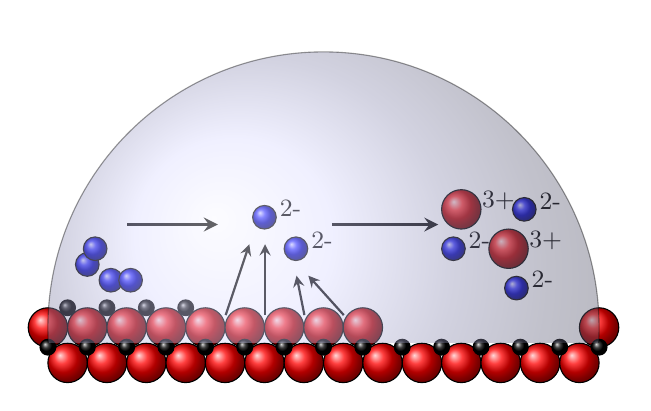
\begin{tikzpicture}[
        >=stealth,
        iron/.style={shade, ball color=red},
        electron/.style={shade, ball color=black},
        oxygen/.style={shade, ball color=blue},
        droplet/.style={ball color=blue!20, opacity=0.4},
    ]

    %Draw the iron atoms
    \foreach \x in {1,1.5,2,2.5,3,3.5,4,4.5,5,8}
            \draw [iron] (\x,1,-0.5) circle (0.25cm);
    \foreach \x in {1.25,1.75,2.25,2.75,3.25,3.75,4.25,4.75,5.25,5.75,6.25,6.75,7.25,7.75}
            \draw [iron] (\x,0.55,-0.5) circle (0.25cm);

    %Draw the iron electrons; this isn't totally realistic for illustrating Fe+3 ions
    \foreach \x in {1.25,1.75,2.25,2.75}
            \draw [electron] (\x,1.25,-0.5) circle (0.1cm);
    \foreach \x in {1,1.5,2,2.5,3,3.5,4,4.5,5,5.5,6,6.5,7,7.5,8}
            \draw [electron] (\x,0.75,-0.5) circle (0.1cm);

    %Draw the O2 molecules
    \draw [oxygen] (1.5,1.8,-0.5) circle (0.15cm);
    \draw [oxygen] (1.6,2.0,-0.5) circle (0.15cm);

    \draw [oxygen] (1.8,1.6,-0.5) circle (0.15cm);
    \draw [oxygen] (2.05,1.6,-0.5) circle (0.15cm);

    %Draw the arrows showing the electrons going to the O2 molecules
    \draw (3.45,1.35) -- (3.75,2.25) [->,thick];
    \draw (3.95,1.35) -- (3.95,2.25) [->,thick];
    \draw (4.45,1.35) -- (4.35,1.85) [->,thick];
    \draw (4.95,1.35) -- (4.5,1.85) [->,thick];

    %Draw O-2 ions with (-) labels
    \shadedraw [oxygen] (3.75,2.4,-0.5) circle (0.15cm) node [above=3pt,right=2pt] {\small{2-}};
    \shadedraw [oxygen] (4.15,2.0,-0.5) circle (0.15cm) node [above=3pt,right=2pt] {\small{2-}};

    %Draw the dissolved Fe+3 ions and O-2 ions
    \shadedraw [iron] (6.25,2.5,-0.5) circle (0.25cm) node [above=3pt,right=4pt] {\small{3+}};
    \shadedraw [iron] (6.85,2.0,-0.5) circle (0.25cm) node [above=3pt,right=4pt] {\small{3+}};

    \shadedraw [oxygen] (6.95,1.5,-0.5) circle (0.15cm) node [above=3pt,right=2pt] {\small{2-}};
    \shadedraw [oxygen] (6.15,2.0,-0.5) circle (0.15cm) node [above=3pt,right=2pt] {\small{2-}};
    \shadedraw [oxygen] (7.05,2.5,-0.5) circle (0.15cm) node [above=3pt,right=2pt] {\small{2-}};

    %Draw the time arrows
    \draw (2.2,2.5) -- (3.35,2.5) [->,very thick];
    \draw (4.8,2.5) -- (6.15,2.5) [->,very thick];

    %Draw the water droplet
    \begin{scope}
            \clip (1,1) rectangle (8.5,5);
            \draw[droplet] (4.5,1,-0.5) circle (3.5cm);
    \end{scope}
\end{tikzpicture}
\end{document}